%%%%%%%%%%%%%%%%%%%%%%%%%%%%%%%%%%%%%%%%%
% Beamer Presentation
% LaTeX Template
% Version 1.0 (10/11/12)
%
% This template has been downloaded from:
% http://www.LaTeXTemplates.com
%
% License:
% CC BY-NC-SA 3.0 (http://creativecommons.org/licenses/by-nc-sa/3.0/)
%
%%%%%%%%%%%%%%%%%%%%%%%%%%%%%%%%%%%%%%%%%

%----------------------------------------------------------------------------------------
% PACKAGES AND THEMES
%----------------------------------------------------------------------------------------

\documentclass{beamer}
% \usepackage{courier}
\usepackage{hyperref}
\usepackage{url}
\usepackage{ulem}
\usepackage{tikz}
\usepackage{multicol}
\usepackage{graphicx}
\usepackage{subcaption}
\usetikzlibrary{fit,calc,positioning,decorations.pathreplacing,matrix}
\usetikzlibrary{positioning}
\usepackage{algorithm}% http://ctan.org/pkg/algorithms
\usepackage{algorithmic}
\usepackage{cleveref}
\usepackage{caption}
\usepackage{appendixnumberbeamer}
\usepackage[latin1]{inputenc}
\usetikzlibrary{shapes, arrows, calc, positioning}

\tikzstyle{block} = [rectangle, draw, fill=blue!20,
    text width=3em, text centered, rounded corners, minimum height=1em, node distance=1.5em, font=\footnotesize]
\tikzstyle{method} = [text width=8em, midway, right]
\tikzstyle{line} = [draw, -latex']
\tikzstyle{edge} = [draw, -, color=red]
\tikzstyle{cloud} = [draw, ellipse, fill=red!20, node distance=1em,
    minimum height=1em]
\tikzstyle{input} = [rectangle, draw,
    text width=3em, text centered, rounded corners, minimum height=1em, node distance=1em]
\tikzstyle{output} = [rectangle, draw,
    text width=3em, text centered, rounded corners, minimum height=1em, node distance=1em]
\tikzstyle{dnn} = [rectangle, draw,  fill=gray!20,
    text width=12em, text centered, rounded corners, minimum height=8em, node distance=1em]

\addtobeamertemplate{navigation symbols}{}{%
    \usebeamerfont{footline}%
    \usebeamercolor[fg]{footline}%
    \hspace{1em}%
    \insertframenumber/\inserttotalframenumber
}
\newcommand{\E}{\text{E}}
\newcommand{\var}{\text{Var}}
\newcommand{\sd}{\text{sd}}

\mode<presentation> {

% The Beamer class comes with a number of default slide themes
% which change the colors and layouts of slides. Below this is a list
% of all the themes, uncomment each in turn to see what they look like.

\usetheme{default}
%\usetheme{AnnArbor}
%\usetheme{Antibes}
%\usetheme{Bergen}
%\usetheme{Berkeley}
%\usetheme{Berlin}
%\usetheme{Boadilla}
%\usetheme{CambridgeUS}
%\usetheme{Copenhagen}
%\usetheme{Darmstadt}
%\usetheme{Dresden}
%\usetheme{Frankfurt}
%\usetheme{Goettingen}
%\usetheme{Hannover}
%\usetheme{Ilmenau}
%\usetheme{JuanLesPins}
%\usetheme{Luebeck}
%\usetheme{Madrid}
%\usetheme{Malmoe}
%\usetheme{Marburg}
%\usetheme{Montpellier}
%\usetheme{PaloAlto}
%\usetheme{Pittsburgh}
% \usetheme{Rochester}
%\usetheme{Singapore}
%\usetheme{Szeged}
%\usetheme{Warsaw}

% As well as themes, the Beamer class has a number of color themes
% for any slide theme. Uncomment each of these in turn to see how it
% changes the colors of your current slide theme.

%\usecolortheme{albatross}
%\usecolortheme{beaver}
%\usecolortheme{beetle}
%\usecolortheme{crane}
%\usecolortheme{dolphin}
%\usecolortheme{dove}
%\usecolortheme{fly}
%\usecolortheme{lily}
%\usecolortheme{orchid}
%\usecolortheme{rose}
%\usecolortheme{seagull}
%\usecolortheme{seahorse}
%\usecolortheme{whale}
%\usecolortheme{wolverine}

%\setbeamertemplate{footline} % To remove the footer line in all slides uncomment this line
%\setbeamertemplate{footline}[page number] % To replace the footer line in all slides with a simple slide count uncomment this line

%\setbeamertemplate{navigation symbols}{} % To remove the navigation symbols from the bottom of all slides uncomment this line
}

\usepackage{graphicx} % Allows including images
\usepackage{booktabs} % Allows the use of \toprule, \midrule and \bottomrule in tables


\usepackage{amsmath}

\newcommand{\red}{\textcolor{red}{red}}
\newcommand{\green}{\textcolor{green}{green}}
\newcommand{\cyan}{\textcolor{cyan}{cyan}}
%----------------------------------------------------------------------------------------
% TITLE PAGE
%----------------------------------------------------------------------------------------


\title{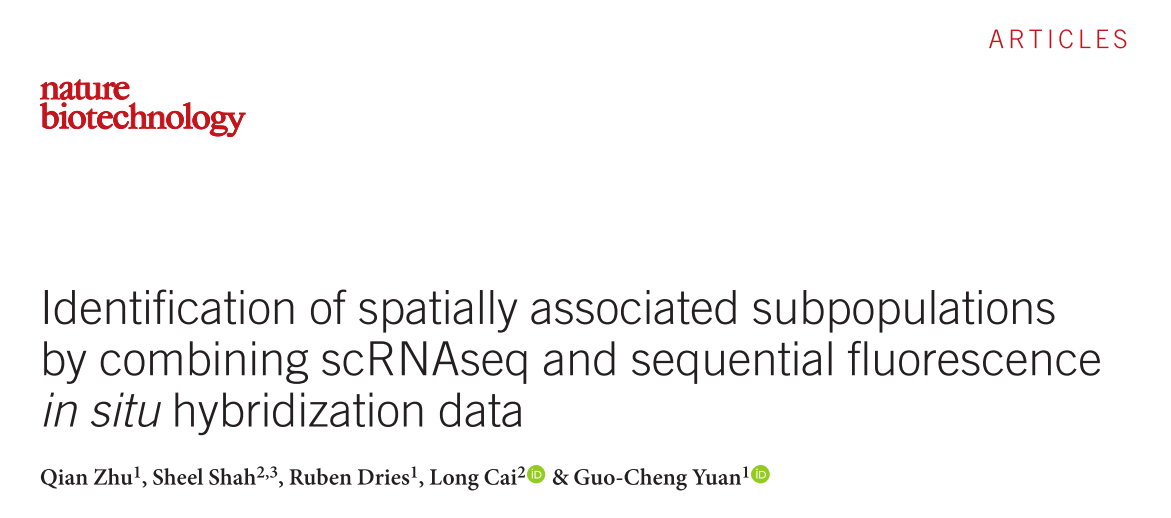
\includegraphics[width=\textwidth]{title}} % The short title appears at the bottom of every slide, the full title is only on the title page
\author{Faculty: Mengjie Chen \& Student: Yanyu Liang}
\institute[]
{
GGSB Journal Club
}
\date{5/2/19} % Date, can be changed to a custom date


\begin{document}

\begin{frame}
\titlepage % Print the title page as the first slide
\end{frame}
\addtocontents{toc}{\setcounter{tocdepth}{1}}
\begin{frame}
\frametitle{Overview} % Table of contents slide, comment this block out to remove it
\tableofcontents % Throughout your presentation, if you choose to use \section{} and \subsection{} commands, these will automatically be printed on this slide as an overview of your presentation
\end{frame}

%----------------------------------------------------------------------------------------
% PRESENTATION SLIDES
%----------------------------------------------------------------------------------------


%------------------------------------------------
\section{Background - On the other side of NGS}
%------------------------------------------------

  \begin{frame}
  \frametitle{FISH and single molecule FISH}
  \begin{itemize}
    \item FISH: what is FISH?
    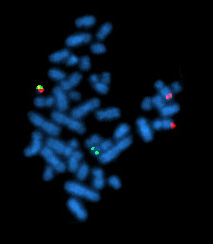
\includegraphics[width=0.4\textwidth]{Bcrablmet}
    \cite{wiki:Fluorescence_in_situ_hybridization}
    \item single molecule FISH: pioneered by \cite{femino1998visualization}, enhanced version by \cite{raj2006stochastic}
  \end{itemize}
  \end{frame}

  \begin{frame}
  \frametitle{Super-resolution microscopy}
  \begin{itemize}
    \item Resolution 10-20 nm on x, y and <50 nm on z direction.
    \item It helps to unreal finer structure (under diffraction barrier)
      \centering
      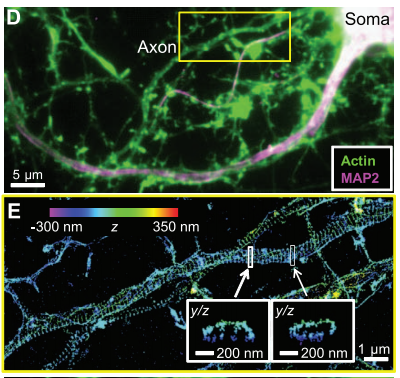
\includegraphics[width=0.5\textwidth]{storm} \cite{xu2013actin}
  \end{itemize}
  \end{frame}

  \begin{frame}
  \frametitle{Sequential FISH}
  \centering
  \begin{itemize}
    \item Encode sequencing with combination of color \cite{lubeck2012single}
    \item Encode sequencing with order of color
    \centering
    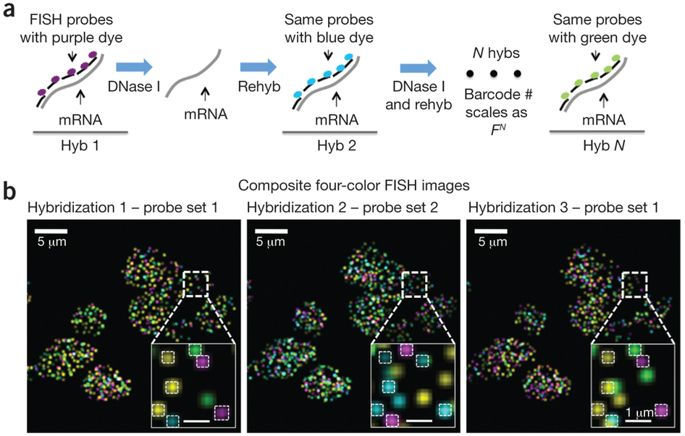
\includegraphics[width=0.5\textwidth]{nmeth_2892_F1} \cite{lubeck2014single}
    \item Sequencing by hybridization, \textit{e.g.} two rounds three channels:
      \begin{itemize}
        \item \red - \cyan $\rightarrow$ Gene 1
        \item \green - \cyan $\rightarrow$ Gene 2
        \item \cyan - \red $\rightarrow$ Gene 3
      \end{itemize}
    \item The complexity of the target library: number of hybridization $\times$ number of channels/probes
  \end{itemize}
  \end{frame}

  \begin{frame}
  \frametitle{What is good about seqFISH?}
  \begin{itemize}
    \item Low drop out rate ($\sim 94\%$ per round), very low probability to have two drop outs
    \item So that it is also easy to correct for this drop out error by one extra round
    \item 84\% efficacy (capture 84\% variation presented in gold standard method smHCR, hybridization chain reaction)
    \item As compared to single-cell RNA-seq, efficacy is 5-20\% (in which step in library preparation it happens?)
  \end{itemize}
  \cite{shah2016situ}
  \end{frame}

  \begin{frame}
  \frametitle{What is good about seqFISH? More importantly?}
  \begin{itemize}
    \item As an in situ technology, it preserves spatial information which is erased in scRNA-seq
  \end{itemize}
  \cite{shah2016situ}
  \end{frame}


%----------------------------------------------------------------------------------------

%------------------------------------------------
\begin{frame}[allowframebreaks]
\frametitle{References}
\footnotesize
\bibliography{ref}
\bibliographystyle{apalike}
\end{frame}

%----------------------------------------------------------------------------------------


\end{document}
